\section{Projektumsetzung}

Die Umsetzung der Anforderungen wird mithilfe der bereitgestellten Hardware und des Tunnels über den Broker Sixxs realisiert. Da nur ein Server zur Verfügung steht, aber Server mit verschiedenen Betriebssystemen genutzt werden sollen, wird auf dem vorhandenen no-name Server ein Hypervisor auf Basis von Ubuntu 16.04 installiert. Über diesen werden zwei virtuelle Server eingerichtet. Der eine wird mit Windows 2012R2 betrieben und der andere ebenfalls mit Ubuntu 16.04. Auf letzterem werden sowohl Mailserver als auch Webserver realisiert. Sollte sich dieser Plan nicht umsetzen lassen, wird der no-name Server rein als Mail- und Webserver verwendet werden. Auf einem der Clients wird dann Windows 2012R2 installiert.

Mithilfe des Cisco Routers wird sowohl die Firewall als auch die Trennung des internen Netzwerkes in zwei Zonen realisiert. Bei den beiden Zonen handelt es sich um eine DMZ, in der sich der Mail- und Webserver befinden werden und um eine Trusted Zone, in der sich die Clients und der Windows-Server befinden werden. Die beiden Netzwerke erhalten jeweils ein eigenes IPv6-Subnetz und werden zudem durch VLANs voneinander getrennt. Die Firewallregeln, Subnetze und VLANs werde im Netzwerkkonzept beschrieben.

\subsection{Skizzierung der Umsetzung}

Die gezeigte Grafik beschreibt die von uns angestrebte, logische Umsetzung der Umgebung. Sowohl die Server als auch die Clients werden über den vorhandenen Cisco Switch verbunden. Der Switch wird per Router mit dem Internet (WAN) verbunden.


\begin{figure}[h]
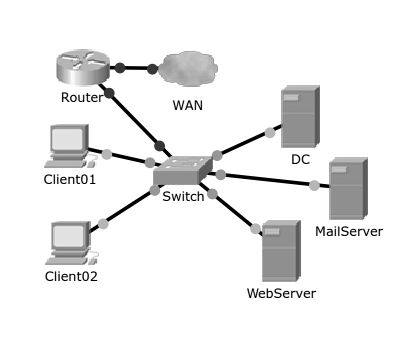
\includegraphics[scale=1]{../8gruppe_packettracer/8gruppe_netzaufbau.png}
\label{skizzierung-umsetzung}
\caption{Skizzierung der Umgebung}
\end{figure}


\subsection{Arbeitspackete}
Liste der geplanten Arbeitspackete\\
\noindent \begin{tabular}{|l|l|}
\hline
AP001 & Zusammentragen und Überprüfen der Hardware \\
AP002 & Router: Basisconfig (IPv6) \\
AP003 & Switch: Basisconfig (IPv6) \\
AP004 & Router: Routing Intern \\
AP005 & Script: Netzwerk Tests \\
AP006 & Test: Netzverfügbarkeit \& Konnektivität \\
AP007 & Test: Netzwerk Reinheit (kein IPv4 / Wireshark) \\
AP008 & Router: SIXXS-Tunnel \\
AP009 & Test: Tunnel Stabilität/Konnektivität/Goodwidth \\
AP010 & Router IPv6 Firewall \\
AP011 & Backup: Router \& Switch Konfiguration \\
AP012 & Installation: Hypervisor \\
AP013 & Konfiguration Hypervisor \\
AP014 & Installation: Linux Server mit LAMP \\
AP015 & Konfiguation: Web-/ Mailserver \\
AP016 & Test: Aufruf Websites intern \\
AP017 & Test: Mailversand intern \\
AP018 & Test: Mailversand nach Draußen \\
AP019 & Test: Webserver Zugriff von Außen \\
AP020 & Test: Firewall (nmap) \\
AP021 & Installation: Windows Domain Controller \\
AP022 & Konfiguration: Windows Domain Controller \\
AP023 & Test: Domänen Verfügbarkeit \\
AP024 & Test: Authentizierung am AD \\
\hline
\end{tabular}
\vspace{0.5cm}\\
Liste der geplanten Zuordnung der Arbeitspackete\\
\noindent \begin{tabular}{|l|c|}
\hline
Tom Vogler & AP001, AP003, AP007, AP011, AP009, AP016, AP017, AP021, AP022 \\
Kilian Engelhardt & AP001, AP005, AP006, AP012, AP013, AP014, AP015, AP023, AP024 \\
Mirko Grossmann & AP001, AP002, AP004, AP008, AP010, AP018, AP019, AP020, AP005 \\
\hline
\end{tabular}
